%----------------------------------------------------------------------------------------
%	Using MATLAB for Data Analysis
%----------------------------------------------------------------------------------------

\chapterimage{chapter_head_1.pdf} % Chapter heading image

\chapter{Using MATLAB for Data Analysis}
MATLAB stands for ``MATrix LABoratory'', which means that the program is on the one hand {\it extremely} good at working with matrices and on the other {\it somewhat limited} to those problems that can be solved using matrices. Naturally, if you spend some money and buy extra toolboxes it can do somewhat more elaborate calculations. In particular, the curve fitting toolbox is excellent and can do most if not all of the data analysis you might encounter in PHY 353L or PHY 474. In general though, if you are thinking about a problem and you can think of a way to quickly solve it using matrices and vectors, MATLAB is a good option. 

\begin{remark}
If you get MATLAB and think you might also buy the curve-fitting toolbox, you should get it at the same time as the main program since Mathworks updates their product very frequently (usually about twice per year), and if you have an academic license you can only get the most recent editions of the toolboxes online.
\end{remark}
\section{Introduction}
Since MATLAB is designed to work predominantly with lab data, it has many features which are tailored specifically to common tasks engineers and experimentalists do on a regular basis. For instance, the program has a file organizing system which can be viewed at any time and graphical user interfaces for common tasks like curve-fitting and importing data. Mathematica, on the other hand, is designed to encompass a much wider range of problems and so often falls short of MATLAB when it comes to convenience and ease of use in a laboratory setting.
\subsection{Scripts -- what makes MATLAB so popular}
When you want to do anything in MATLAB, you will always either use the buttons in the menus, or you will execute expressions through the `Command Window'. Because the expressions you might want to execute might be complicated and long, MATLAB has a file type (`.m') that it interprets as a long chain of commands. This is called a \emph{script} and is used widely in the MATLAB community to do a wide variety of computations.
When you open MATLAB you will see a few open `panes' in the program.
\begin{itemize}
\item{\bf Current Folder} -- This is where MATLAB looks for anything new (data, functions, scripts). If you're trying to load data make sure the `Current Folder' is looking at the file you're trying to use.
\item{\bf Editor} -- This is where you can edit and create new scripts and functions.
\item{\bf Workspace} -- This is the pane that displays all variables and their basic characteristics. This is very useful for checking up on variable characteristics.
\item{\bf Command Window} -- This is where expressions are executed. The most common things are functions, commands, and scripts.
\item{\bf Command History} -- This is where past expressions are stored so that you can access them easily. One very useful trick while coding in MATLAB is to press the `up' key on the keyboard to access the last command so you can edit it without having to write it out again.
\end{itemize}

The easiest ways to make a new script are (1) to press \texttt{Ctrl+N} while in the editor or (2) right-click on the Current Folder window and choose the `New File $\to$ Script' option. Once you have a \texttt{filename.m} file up, you can execute the entire file by simply typing \texttt{filename} in the command window.
\subsection{Syntax \& functions}

In MATLAB, commands \& functions are executed from the `command window'. Functions are of the form \texttt{functionName($arguments$)} in which case they call the \texttt{functionName} \emph{function}; commands are of the form \texttt{command $argument$}, in which case they run the \texttt{command} \emph{command}. In MATLAB, function inputs are always separated with commas and command inputs are always separated with spaces. Code is always interpreted in this way, which makes it easy to read. 
For instance:
\begin{example}[Command syntax]
\hfill \\
Some common examples of command syntax:
\begin{enumerate}
\item \texttt{clear all -except var1} clears all variables except for the variable named \texttt{var1}.
\item \texttt{load filename.mat} loads the variables saved to the {filename.mat} file.
\item \texttt{disp `This is a sentence which is also a string'} displays the sentence: \texttt{This is a sentence which is also a string}
\end{enumerate}
\end{example}

\begin{example}[Function syntax]
\hfill \\
Some common examples of function syntax:
\begin{enumerate}
\item \texttt{plot(x,y)} plots the vector \texttt{x} against the vector \texttt{y}, connecting each successive pair of points with a line segment \emph{note:} these vectors must be the same size.
\item \texttt{scatter(x,y)} plots the vector \texttt{x} against the vector \texttt{y} in a scatter plot, rather than connecting points.
\item \texttt{disp(a)} displays the object \texttt{a}, which might be a string, a matrix or some other object.
\end{enumerate}
\end{example}

To make a comment, just as in \LaTeX , you put a \texttt{\%} sign at some point in a line. Everything after that \texttt{\%} sign but before the next line gets commented out.
\begin{example}[Comments and displaying variables]
\hfill \\
Running the script:
\begin{framed}
\begin{verbatim}
% This is a comment and will not be displayed
a = [ 1 2 ; 4 5; 7 8]; % the matrix describing something important
b = [ 1 2 7 8]; % a vector  describing something important
disp 'The important matrix is:'; 	disp(a);
disp 'The important vector is:'; 	b
\end{verbatim}
\end{framed}
yields the output:
\begin{framed}
\begin{verbatim}
The important matrix is:
     1     2
     4     5
     7     8

The important vector is:

b =

     1     2     7     8
\end{verbatim}
\end{framed}
 In this way, you can get a script to output the answer to a calculation in a convenient format.
\end{example}


\subsection{Loading data}\label{loadingdata}
When you open the program, you will see a box on the left titled `Current Folder'. MATLAB can only see the files in your current folder, so this is where all your data files should go. Once a data file is in that folder, you can simply right-click the file and say `Import Data...'. Alternatively, you can go to the `File' menu and choose `Import Data...'. In either case you will end up in the same import wizard. You will be previewing the data to make sure it is in the right format. MATLAB is usually pretty good about identifying what kind of data you have (e.g. `comma-separated' or `tab-delimited'). 
Once you have your data imported into a matrix (the most convenient) or into a collection of differently named vectors, you can save the workspace into what is called a \texttt{.mat} file. This is MATLAB's special file format for saving workspaces. Now whenever MATLAB's current folder contains the your \texttt{data.mat} (assuming you named it \texttt{data.mat}), you can just use the \texttt{load data} command to import all the data that was in your workspace when you saved it.

\begin{exercise}[Importing multiple files ]
If you have a lot of files of the same type and you want them all to import the same way, one way to do that is to check the `Generate MATLAB Code' box in the import wizard. What this does is generate the code to import data of the form you specified in the prompt. If you save this code as `importfile' once it comes up, you will be able to use this command to import files quickly and reliably in a script.

This way you don't have to click through the wizard $n$ times if you have $n$ data files.%
\end{exercise}
\subsection{Plotting functions and data}
While in Mathematica, it is easy to tell the computer to plot a function against a dependent variable (or some other function of a dependent variable), MATLAB only understands vectors. This means that to plot $\sin(x)$ against $x$ for instance, you need to first decide which $x$ points you want. After you have an independent variable vector, and have the ability to construct a dependent variable vector (or if you already have two vectors of the same length), you can easily make a plot by calling the \verb|plot(xdata,ydata)| function.
\begin{framed}
\begin{verbatim}
x = 0:1e-2:2*pi;
plot(x,sin(x));
\end{verbatim}
\end{framed}
In the above code, the statement \verb| x = 0:1e-2:2*pi;| creates a vector of increasing values starting at \verb|0| and working up in increments of \verb|1e-2| ($1 \times 10^{-2}$) until the point \verb|2*pi|$=2\pi$ is reached. Again, once the domain of the function is created, it is easy to simply apply the sine function while creating the \texttt{plot()}. Note that a semicolon has been placed after each line -- the first is to keep the variable \verb|x| from being displayed, the second is for aesthetics. In general there's no harm in putting down a semicolon so use them everywhere.
\begin{figure}[H]
\centering
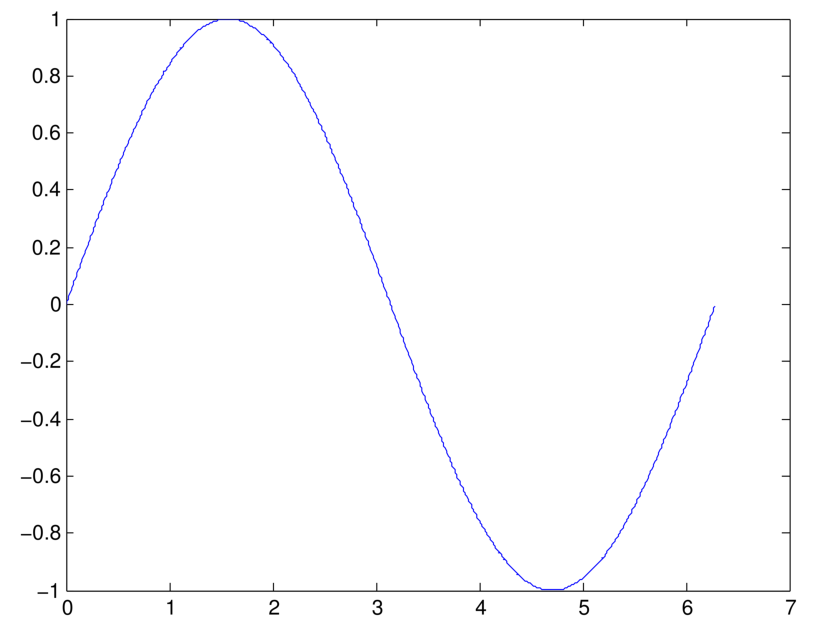
\includegraphics[scale=1]{sinplot.pdf}
\caption{Plot of \texttt{sin(x)} against \texttt{x}, where \texttt{x} is a $ 1 \times 629 $ vector from 0 to $2\pi$.}
\end{figure}
To plot data, it is often most convenient to have all your data in a matrix. It is a good practice to document your variables and how you name them somewhere. Documenting how the code you write is relevant to the experiment can easily be done with comments in the same file as your analysis using \texttt{\%} to create comments just as in \LaTeX. In the code below, the data has already been imported using the import data wizard mentioned 
in section \ref{loadingdata} and titled \texttt{data}. Fig. \ref{dataplot} shows the result:

\begin{framed}
\begin{verbatim}
plot(data(:,1),data(:,2));
xlabel('Column 1');
ylabel('Column 2');
title('Column 1 vs. Column 2');
\end{verbatim}
\end{framed}
\begin{figure}[h]
\centering
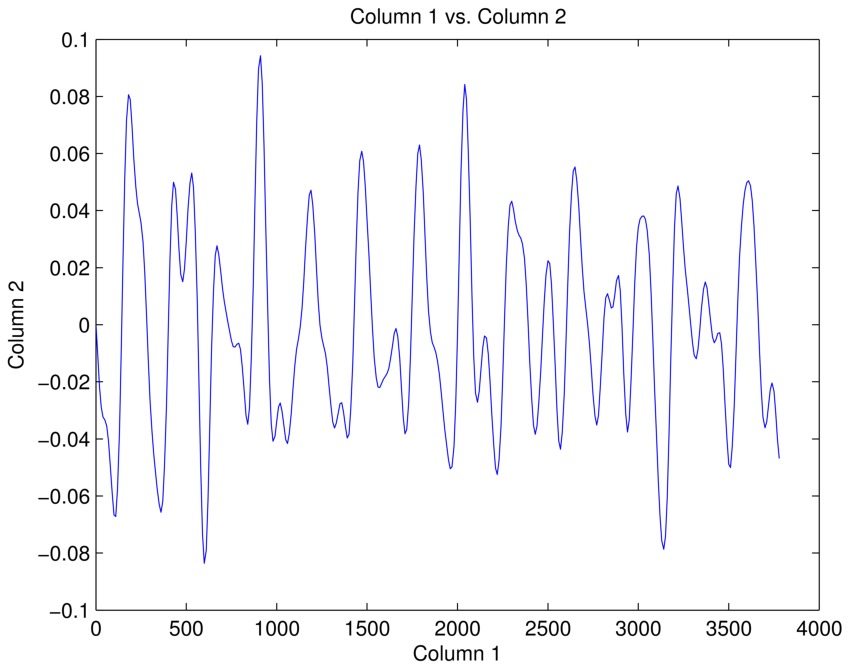
\includegraphics[scale=1]{p1e1.pdf}
\caption{Plot of one column of data (\texttt{data(:,1)}) against another (\texttt{data(:,2)}).}
\label{dataplot}
\end{figure}
This is the most basic kind of plot. However, often you may want to plot your data as points (in a scatter plot), rather than as a line plot. MATLAB has another function called \texttt{scatter()} which for two vectors works in exactly the same way as \texttt{plot()}. As in Mathematica, these functions are highly customizable.
\begin{remark}
In MATLAB there's a very nice way to customize plot which so long as you only have one plot is very easy and efficient. It is called the \emph{property editor}. You can get to it via the view menu if you have a plot open. It is a graphical user interface (GUI) with many options for titling plots, changing colors, sizes, line styles, etc.
\end{remark}

\subsection{Saving pictures}

If you're happy with your plot and want to put it into your paper you must first export it by going to \emph{Export Setup}. You can get to export setup through ``File $\to$ Export Setup" if you have an element on the figure selected in the Property Editor, or in the Property Editor window.\\

\emph{Remember:} you want to export files in the .pdf or .eps format as those do not have problems scaling when incorporated into a \LaTeX\ document.

\subsection{Histograms}

To make a histogram of a vector or matrix of data, the simplest thing is simply to write \texttt{hist(data)}. This will create a histogram plot with a number of bins that MATLAB thinks is appropriate. However, you can specify the number of bins with \texttt{hist(data,bins)} and if you would like to plot the bin centers against the bin counts, you can assign the output of the \texttt{hist} to two vectors representing this as in the example below:

\begin{framed}
\begin{verbatim}
[count, bin] = hist(data(:,2),30);
subplot(2,1,1); plot(bin,count);
title('Plot from Histogram Output');
subplot(2,1,2); hist(data(:,2),30);
title('Regular Histogram Plot');
\end{verbatim}
\end{framed}

\begin{figure}[h]
\centering
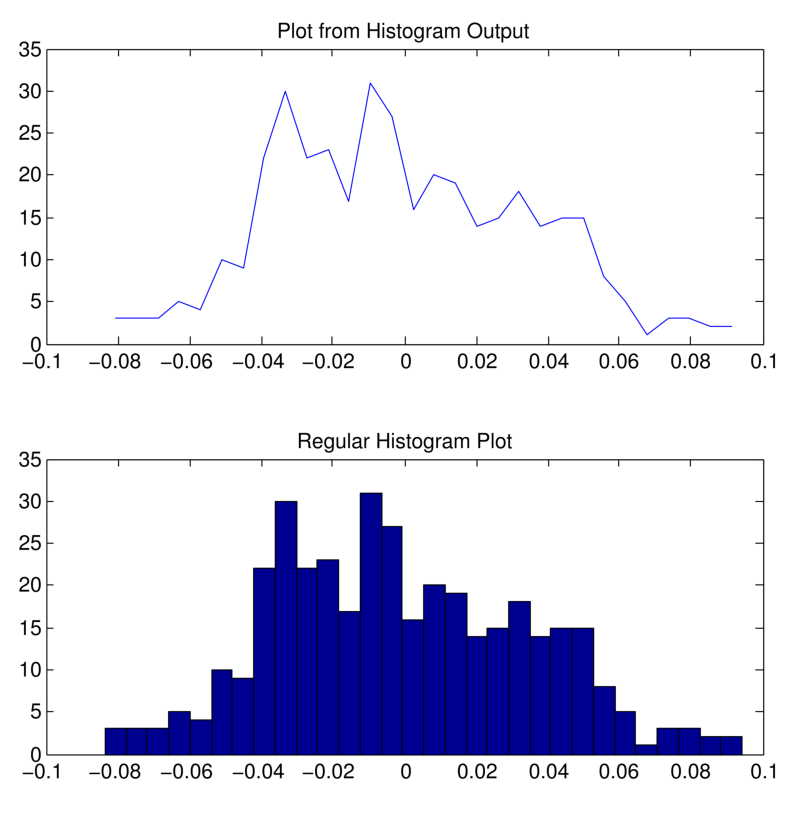
\includegraphics[scale=1]{histexample.pdf}
\caption{{Plots of the same histogram portrayed in two different ways. (Top) Histogram data is stored in two variables (\texttt{[count, bin]}) from the  \texttt{hist(data(:,2),30);} command which is a 30 bin histogram on \texttt{data(:,2)}. (Bottom) The traditional histogram from \texttt{hist(data(:,2),30);}. As you can see, \texttt{hist(data(:,2),30);} automatically outputs a plot unless you get output data from the function. If you were interested in how the data were distributed,\texttt{ [count, bin] = hist(data(:,2),30);} would be most useful because you could fit the \texttt{bin} and \texttt{count} with some distribution function (a gaussian for instance).}}
\label{histoplot}
\end{figure}
